

  % begin the content of the document
\sloppy  % this to relax whitespacing in favour of straight margins



% title on top of the document
\maintitle{Kale-ab Tessera}{December 8,1994}{Last update on \today}

\nobreakvspace{0.3em}  % add some page break averse vertical spacing

\noindent\href{mailto:kaleabtessera.at.gmail.dot.com}{kaleabtessera\mbox{}@\mbox{}gmail.com}\sbull
\textsmaller{+}27.766806878\sbull
\\
House Boekenhout\sbull
LC de Villiers Campust\sbull
Hatfield\sbull
Pretoria\\

\spacedhrule{0.9em}{-0.4em}  % a horizontal line with some vertical spacing before and after
\begin{center}
\roottitle{Summary}  % a root section title
\end{center}


\vspace{-1.3em}  % some vertical spacing
\begin{multicols}{3}% open a multicolumn environment

\noindent 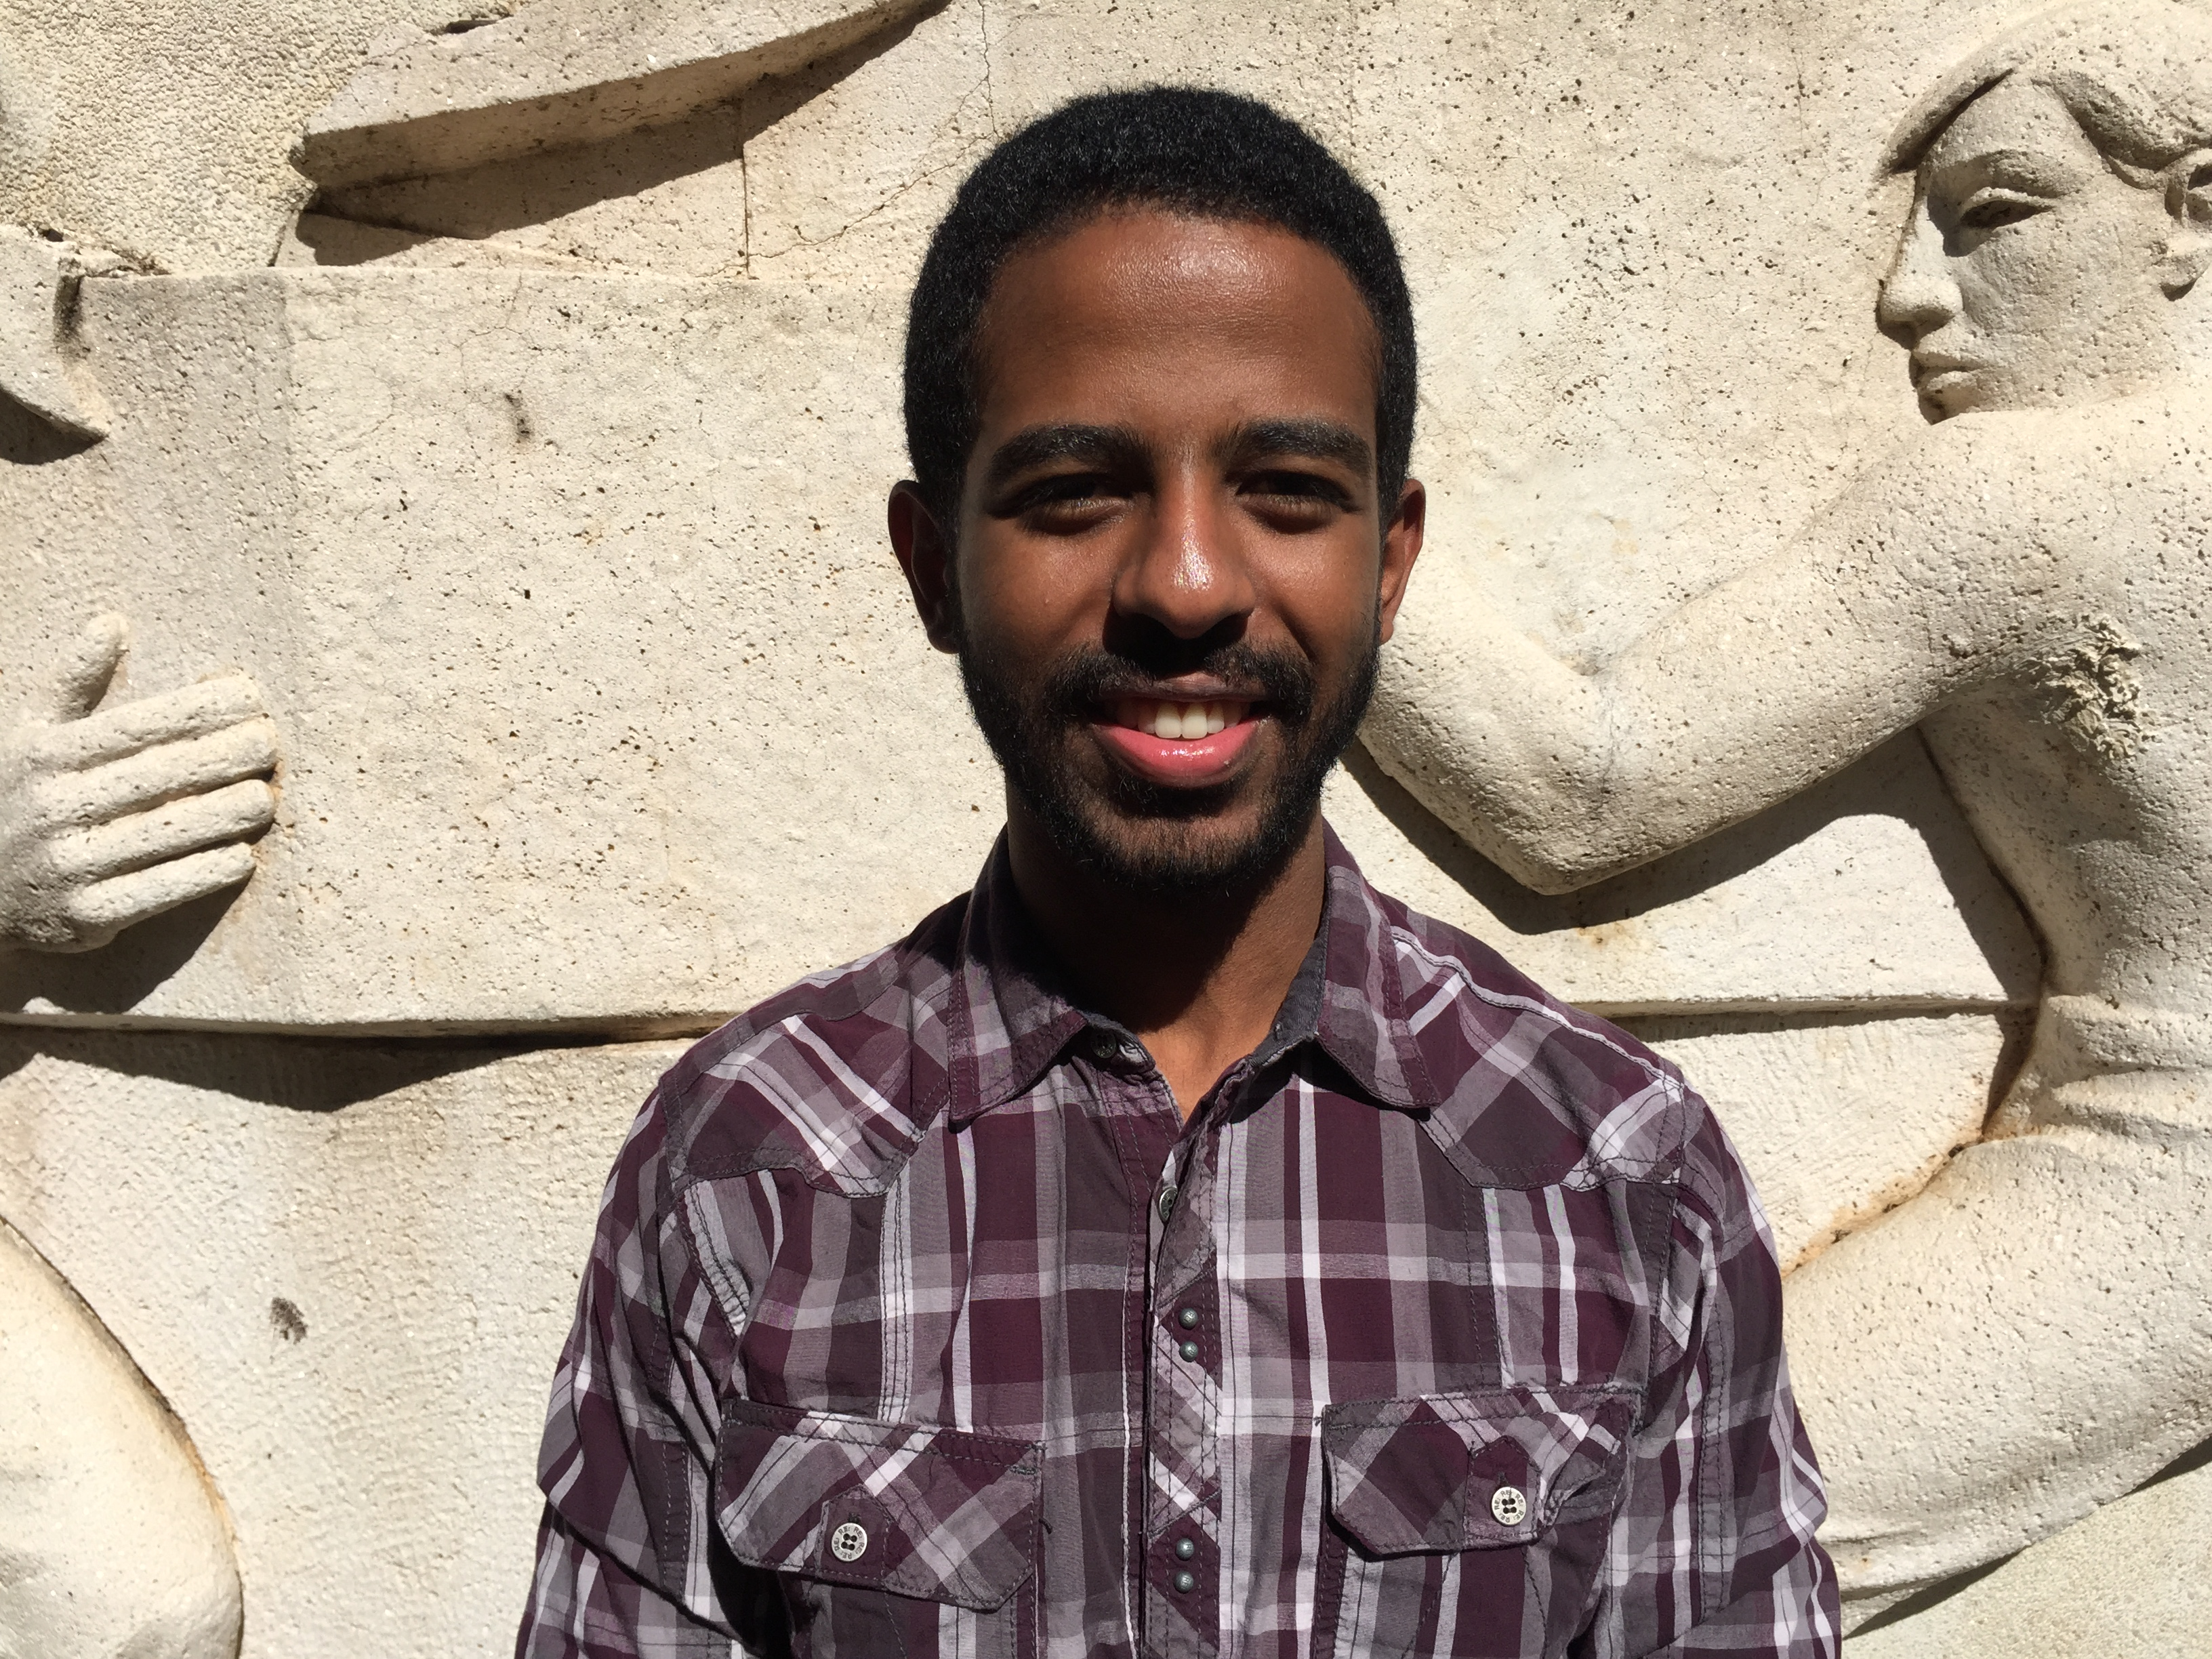
\includegraphics[width=\linewidth]{kaleab}\\Ambitious programmer with strong leadership and relationship skills. Adaptable and very open to learning new programming languages and methodologies, in order to build on previous knowledge. Hardworking yet still innovative. I try to live a live with as many experiences as possible cause I believe we can only learn and grow from things that challenge us. I am uncomfortable in my comfort zone. 

\end{multicols}

\spacedhrule{0em}{-0.4em}

\roottitle{Experience}
\headedsection  % sets the header for the section and includes any subsections
  {\href{http://www.cs.up.ac.za}{University of Pretoria, Computer Science Department}}
  {\textsc{Hatfield, Pretoria}} {%
  \headedsubsection
    {Teaching Assistant - COS 110}{july14 -- dec 14}
    {\bodytext{As a teaching assistant for Program design and Programming techniques good knowledge of 
 object-oriented (OO) programming. Concepts including inheritance and multiple inheritance, polymorphism, operator overloading, memory management (static and dynamic binding), interfaces and  encapsulation.\\}}
    }
    
\headedsection  % sets the header for the section and includes any subsections
  {\href{http://www.cs.up.ac.za}{University of Pretoria, Computer Science Department}}
  {\textsc{Hatfield, Pretoria}} {%
  \headedsubsection
    {Teaching Assistant - COS 212}{feb 14 --  present}
    {\bodytext{As a teaching assistant for Data Structures and Algorithms it was crucial to identify and recognise all the classical data structures; implement them in different ways; know how to measure the efficiency of implementations and algorithms; and have
further developed their programming skills, especially with recursion and polymorphism.\\}}
    }
    
\headedsection  % sets the header for the section and includes any subsections
  {\href{http://www.up.ac.za/boekenhout}{Boekenhout Res}}
  {\textsc{Hyde Park, Johannesburg}} {%
  \headedsubsection
    {House Committee Member, Secretary, Head of IT and Communications   }
    {aug 14 – present}
    {\bodytext{Helped lead various res students and mentored those with difficulties. I was also expected to solve technical 
dificulties such as problems connecting to the internet and also managing of social media. \\}}
}
    
\spacedhrule{-0.2em}{-0.4em}


\roottitle{Technical Skills}

\inlineheadsection  % special section that has an inline header with a 'hanging' paragraph
  {Technical expertise:}
  {Proficient in Java, C++ and html. Experience with Assembly ,C, sql and delphi. Well-equipped in data structures and algorithms}

\vspace{0.5em}
\inlineheadsection
  {Natural languages:}
  {English \emph{(full professional proficiency)}}


\spacedhrule{1.6em}{-0.4em}

\roottitle{Interests}
\inlineheadsection
  {Non-exhaustive:}
  {Keeping fir, playing tennis and soccer, dancing, cooking, technology trends , music, foreign cultures, software development and application of artificial intelligence}

  
\spacedhrule{1.6em}{-0.4em}  
  
\roottitle{Non - Technical Strengths}

\inlineheadsection
  {Social skills:}
  {I believe I am a born-leader and this has resulted in various leadership positions whether it be highschool, residence or the university. I am also quite easy to get along with due to my friendlyness and communication skills.}
  
\inlineheadsection
  {Professional skills:}
  {In a professional working environment I am self-driven and willing to work as hard as is required. I also strive to be very respectful,punctual and diligent in anything that I do.}
  
\spacedhrule{1.6em}{-0.4em}  
  
\roottitle{Why CSIR Ironman Image Throw Thingy?}

\inlineheadsection
  {Because:}
  {Not only am I interested in the obvious visual factors of this project, I am also interested in incorporating various technologies together. This project will be a challenge, but a rewarding one. Once completed, it will be used lecturers. Students and even for recreational purposes like watching movies. I want to be involved in working with software which has so much to offer the world. }